\begin{figure}[!h]
	\begin{minipage}[b]{1.0\linewidth}
		\centering
		\centerline{ 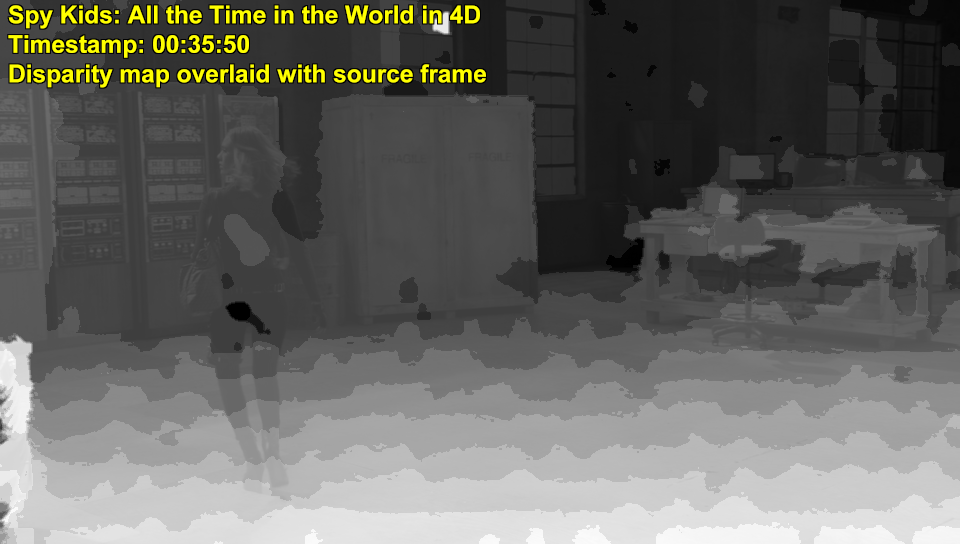
\includegraphics[width=0.7\textwidth]{example_depth} }
	\end{minipage}
	\begin{minipage}[b]{1.0\linewidth}
		\centering
		\centerline{ 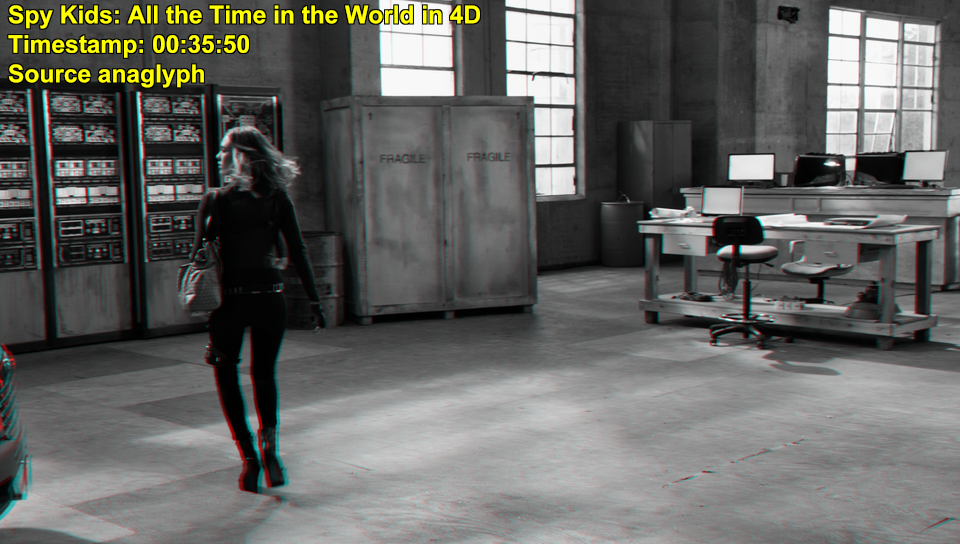
\includegraphics[width=0.7\textwidth]{example_anaglyph} }
	\end{minipage}
    \caption{Пример найденной с помощью предлагаемого метода сцены, содержащей дефект: объект переднего плана оказался слитым с фоном. Создатели фильма забыли нарисовать тело актрисы на карте глубины, поэтому сцена демонстрирует невозможную ситуацию и может вызвать визуальный дискомфорт. На верхнем изображении показана карта диспаратности поверх исходного ракурса, на нижнем --- исходная сцена в анаглифе. }
	\label{fig:example}
\end{figure}
